


\tikzset{every picture/.style={line width=0.75pt}} %set default line width to 0.75pt        

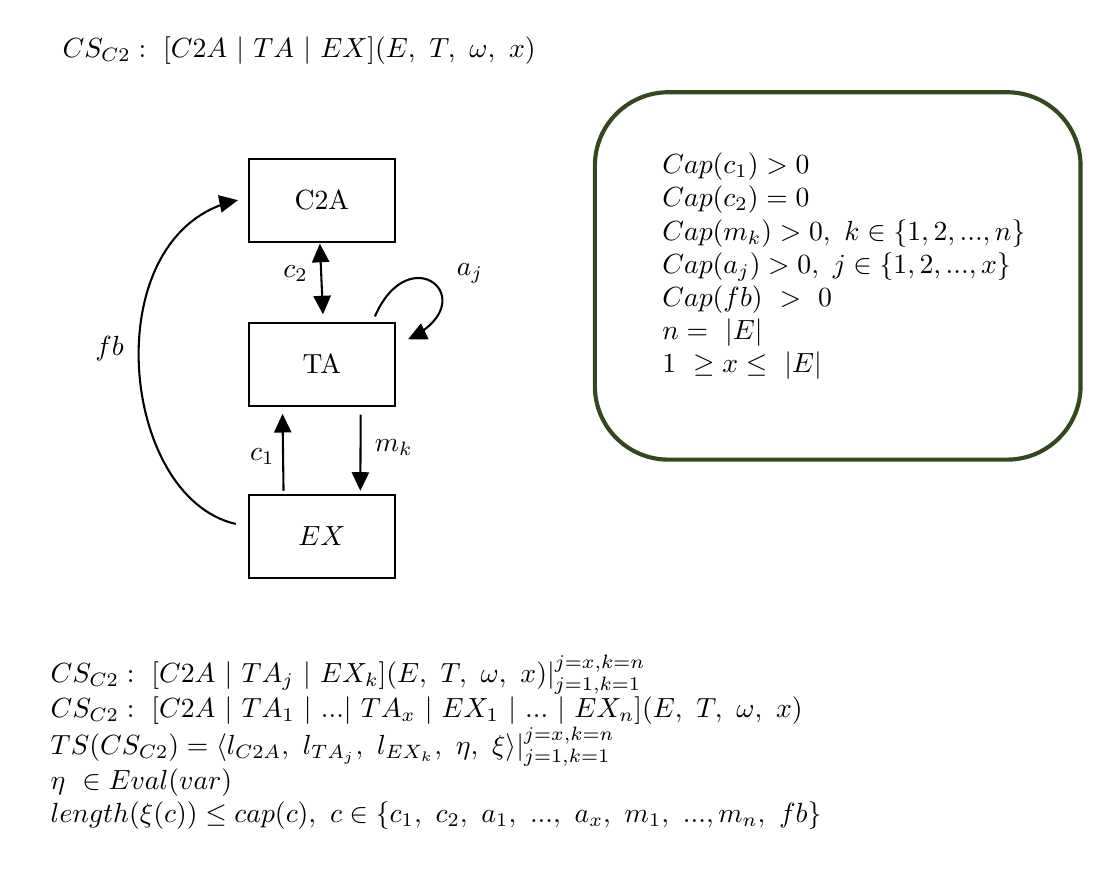
\begin{tikzpicture}[x=0.75pt,y=0.75pt,yscale=-1,xscale=1]
%uncomment if require: \path (0,434); %set diagram left start at 0, and has height of 434

%Shape: Rectangle [id:dp7793135649662085] 
\draw   (146,144) -- (216,144) -- (216,184) -- (146,184) -- cycle ;
%Shape: Rectangle [id:dp8388066725390221] 
\draw   (146,65) -- (216,65) -- (216,105) -- (146,105) -- cycle ;
%Shape: Rectangle [id:dp48691256180587716] 
\draw   (146,227) -- (216,227) -- (216,267) -- (146,267) -- cycle ;
%Straight Lines [id:da3337977868298102] 
\draw    (180.13,109) -- (181.37,137) ;
\draw [shift={(181.5,140)}, rotate = 267.47] [fill={rgb, 255:red, 0; green, 0; blue, 0 }  ][line width=0.08]  [draw opacity=0] (8.93,-4.29) -- (0,0) -- (8.93,4.29) -- cycle    ;
\draw [shift={(180,106)}, rotate = 87.47] [fill={rgb, 255:red, 0; green, 0; blue, 0 }  ][line width=0.08]  [draw opacity=0] (8.93,-4.29) -- (0,0) -- (8.93,4.29) -- cycle    ;
%Straight Lines [id:da7136052167478543] 
\draw    (199.67,188.33) -- (199.51,222) ;
\draw [shift={(199.5,225)}, rotate = 270.26] [fill={rgb, 255:red, 0; green, 0; blue, 0 }  ][line width=0.08]  [draw opacity=0] (8.93,-4.29) -- (0,0) -- (8.93,4.29) -- cycle    ;
%Straight Lines [id:da1199439366931846] 
\draw    (162.5,225) -- (162.04,191) ;
\draw [shift={(162,188)}, rotate = 449.23] [fill={rgb, 255:red, 0; green, 0; blue, 0 }  ][line width=0.08]  [draw opacity=0] (8.93,-4.29) -- (0,0) -- (8.93,4.29) -- cycle    ;
%Rounded Rect [id:dp3574279176331121] 
\draw  [color={rgb, 255:red, 53; green, 71; blue, 31 }  ,draw opacity=1 ][line width=1.5]  (312.5,68.4) .. controls (312.5,48.85) and (328.35,33) .. (347.9,33) -- (511.1,33) .. controls (530.65,33) and (546.5,48.85) .. (546.5,68.4) -- (546.5,174.6) .. controls (546.5,194.15) and (530.65,210) .. (511.1,210) -- (347.9,210) .. controls (328.35,210) and (312.5,194.15) .. (312.5,174.6) -- cycle ;
%Curve Lines [id:da7275055445236782] 
\draw    (139.5,241) .. controls (83.07,228.13) and (71.72,101.57) .. (138.45,85.45) ;
\draw [shift={(140.5,85)}, rotate = 528.53] [fill={rgb, 255:red, 0; green, 0; blue, 0 }  ][line width=0.08]  [draw opacity=0] (8.93,-4.29) -- (0,0) -- (8.93,4.29) -- cycle    ;
%Curve Lines [id:da0050482038741132] 
\draw    (206.5,141) .. controls (223.16,102.78) and (259.03,132.75) .. (224.69,150.9) ;
\draw [shift={(222.5,152)}, rotate = 334.65] [fill={rgb, 255:red, 0; green, 0; blue, 0 }  ][line width=0.08]  [draw opacity=0] (8.93,-4.29) -- (0,0) -- (8.93,4.29) -- cycle    ;

% Text Node
\draw (181,85) node   [align=left] {C2A};
% Text Node
\draw (181,164) node   [align=left] {TA};
% Text Node
\draw (181,247) node    {$EX$};
% Text Node
\draw (152.33,208.33) node    {$c_{1}$};
% Text Node
\draw (215.67,204) node    {$m_{k}$};
% Text Node
\draw (168.33,120.33) node    {$c_{2}$};
% Text Node
\draw (432.5,117) node    {$ \begin{array}{l}
Cap( c_{1})  >0\\
Cap( c_{2}) =0\\
Cap( m_{k})  >0,\ k\in \{1,2,...,n\}\\
Cap( a_{j})  >0,\ j\in \{1,2,...,x\}\\
Cap( fb) \  >\ 0\\
n=\ |E|\ \\
1\ \geq x\leq \ |E|
\end{array}$};
% Text Node
\draw (78.67,156.67) node    {$fb$};
% Text Node
\draw (170,13) node    {$CS_{C2} :\ [ C2A\ |\ TA\ |\ EX]( E,\ T,\ \omega ,\ x)$};
% Text Node
\draw (252.33,120.33) node    {$a_{j}$};
% Text Node
\draw (236,347) node    {$ \begin{array}{l}
CS_{C2} :\ [ C2A\ |\ TA_{j} \ |\ EX_{k}]( E,\ T,\ \omega ,\ x) |^{j=x,k=n}_{j=1,k=1}\\
CS_{C2} :\ [ C2A\ |\ TA_{1} \ |\ ...|\ TA_{x} \ |\ EX_{1} \ |\ ...\ |\ EX_{n}]( E,\ T,\ \omega ,\ x)\\
TS( CS_{C2}) =\langle l_{C2A} ,\ l_{TA_{j}} ,\ l_{EX_{k}} ,\ \eta ,\ \xi \rangle |^{j=x,k=n}_{j=1,k=1}\\
\eta \ \in Eval( var)\\
length( \xi ( c)) \leq cap( c) ,\ c\in \{c_{1} ,\ c_{2} ,\ a_{1} ,\ ...,\ a_{x} ,\ m_{1} ,\ ...,m_{n} ,\ fb\}
\end{array}$};


\end{tikzpicture}
